% ----------------------------------------------------------
% Capítulo 3
% ----------------------------------------------------------
\chapter{Plano de Melhoria da Confiabilidade e Percepção do Cliente}
\label{chap:confiabilidade-feedback}

A confiabilidade e a percepção positiva do cliente são cruciais para o sucesso do VOEBEM. Este plano descreve as práticas de Engenharia de Confiabilidade de Sites (SRE - Site Reliability Engineering) que propomos para alcançar e manter altos níveis de serviço, alinhando a operação técnica com a experiência do cliente.

\section{Monitoramento e Observabilidade}
\label{sec:monitoramento}

Uma estratégia robusta de monitoramento e observabilidade é fundamental para entender o comportamento do sistema, detectar problemas proativamente e garantir que as metas de negócio sejam atendidas. Propõe-se uma abordagem baseada nos três pilares da observabilidade: métricas, logs e traces.

\subsection{SLIs (Service Level Indicators) Chave}
\label{subsec:slis}
Indicadores quantitativos que medem aspectos específicos do serviço. Exemplos para VOEBEM:

\begin{table}[htbp]
    \centering
    \caption{Exemplos de SLIs para o Sistema VOEBEM}
    \label{tab:slis}
    \rowcolors{2}{gray!10}{white} % Adiciona cores alternadas (requer \usepackage[table]{xcolor})
    % Usar tabularx e booktabs. Remover linhas verticais.
    \begin{tabularx}{\textwidth}{lX} % Removido '|'
        \toprule % Substitui \hline
        \textbf{Categoria} & \textbf{SLI (Indicador)} \\
        \midrule % Substitui \hline
        Disponibilidade & \% de requisições bem-sucedidas (HTTP 2xx/3xx) na API Gateway (endpoints chave) \\
        Disponibilidade & \% de requisições bem-sucedidas nas APIs (Reservas, Voos) \\
        Latência & Tempo de resposta (p95, p99) para busca de voos na API Gateway \\
        Latência & Tempo de resposta (p95) para criação de reserva na API de Reservas \\
        Taxa de Erros & \% de requisições com erro (HTTP 5xx) nas APIs (Gateway, Reservas, Voos) \\
        Taxa de Erros & Taxa de falhas na integração com Sistema de Pagamentos \\
        Taxa de Erros & Taxa de erros na publicação/consumo de mensagens (Sistema de Mensageria) \\
        Saturação & Uso de CPU/Memória dos containers \\
        Saturação & Uso de conexões do banco de dados \\
        Saturação & Profundidade da fila no Sistema de Mensageria \\
        \bottomrule % Substitui \hline
    \end{tabularx}
\end{table}

\subsection{SLOs (Service Level Objectives)}
\label{subsec:slos}
Metas claras e mensuráveis para os SLIs mais críticos, definindo o nível de serviço esperado. Exemplos:

\begin{table}[htbp]
    \centering
    \caption{Exemplos de SLOs para o Sistema VOEBEM}
    \label{tab:slos}
    \rowcolors{2}{gray!10}{white}
    % Usar tabularx e booktabs.
    \begin{tabularx}{\textwidth}{XXl} % Removido '|'
        \toprule
        \textbf{SLI Referente} & \textbf{Exemplo de SLO (Meta)} & \textbf{Janela} \\
        \midrule
        Disponibilidade API Gateway (Busca/Reserva) & >= 99.9\% de requisições bem-sucedidas & Mensal \\
        Latência Busca de Voos (p95) & < 800ms & Contínua \\
        Latência Criação de Reserva (p95) & < 1500ms & Contínua \\
        Taxa de Erros API Reservas (5xx) & < 0.1\% & Mensal \\
        \bottomrule
    \end{tabularx}
    \par\medskip
    \textit{(Nota: Estes são exemplos iniciais e devem ser refinados com base em dados históricos e necessidades de negócio).}
\end{table}

\subsection{Ferramentas Propostas}
\label{subsec:monitoramento-ferramentas}

\begin{table}[htbp]
    \centering
    \caption{Ferramentas Propostas para Monitoramento e Observabilidade}
    \label{tab:monitoramento-ferramentas}
    \rowcolors{2}{gray!10}{white}
    % Usar tabularx e booktabs.
    \begin{tabularx}{\textwidth}{lXX} % Removido '|'
        \toprule
        \textbf{Pilar} & \textbf{Ferramenta(s) Proposta(s)} & \textbf{Principal Responsabilidade} \\
        \midrule
        Métricas & Prometheus + Grafana & Coleta e Visualização de Métricas (SLIs, SLOs, Saúde) \\
        Logs & Fluentd/Bit + Loki + Grafana (ou ELK Stack) & Coleta, Agregação e Consulta de Logs \\
        Tracing & Jaeger + OpenTelemetry + Grafana & Coleta e Visualização de Traces Distribuídos \\
        Alertas & Alertmanager + PagerDuty/Opsgenie & Definição de Regras de Alerta e Notificação On-Call \\
        \bottomrule
    \end{tabularx}
\end{table}

\subsection{Alertas}
\label{subsec:alertas}
\begin{itemize}
    \item Configurados no \textbf{Alertmanager} (parte do ecossistema Prometheus).
    \item Baseados principalmente na \textbf{violação dos SLOs} (Exemplo: taxa de erro acima do limite por X minutos, latência p99 excedendo o objetivo) ou em \textbf{sintomas críticos} (Exemplo: serviço indisponível, erro de acesso ao banco de dados, fila de mensagens crescendo rapidamente, certificados expirando).
    \item Alertas devem ser \textbf{acionáveis}, indicando claramente o problema e o impacto potencial.
    \item Direcionamento para a equipe de plantão (on-call) através de ferramentas como \textbf{PagerDuty} ou \textbf{Opsgenie}, com diferentes níveis de severidade e canais de notificação (Exemplo: chat, telefone).
\end{itemize}

\section{Automação de Recuperação}
\label{sec:automacao-recuperacao}

Para aumentar a resiliência e reduzir a necessidade de intervenção manual em caso de falhas, propõe-se a implementação de mecanismos de recuperação automática, principalmente aproveitando recursos do Kubernetes e serviços gerenciados na nuvem.

\subsection{Auto-Healing (Kubernetes)}
\label{subsec:auto-healing}
\begin{itemize}
    \item \textbf{Liveness Probes:} Verificações periódicas configuradas nos Deployments/StatefulSets. Se um container falhar na verificação (Exemplo: travado, não respondendo a um endpoint \texttt{/healthz}), o Kubelet o reiniciará automaticamente na mesma instância (Node).
    \item \textbf{Readiness Probes:} Verificações que indicam se um container está pronto para receber tráfego (Exemplo: aplicação iniciada, conexões estabelecidas). O Kubernetes só enviará tráfego (via Services) para Pods que estejam "Ready". Se um Pod falhar na Readiness Probe, ele é temporariamente removido do balanceamento de carga até se recuperar.
    \item \textbf{ReplicaSets/Deployments:} Garantem que o número desejado de réplicas de um serviço esteja sempre em execução. Se um Node falhar, os Pods que estavam nele são automaticamente reagendados em outros Nodes saudáveis.
\end{itemize}

\subsection{Auto-Scaling (Kubernetes)}
\label{subsec:auto-scaling}
\begin{itemize}
    \item \textbf{Horizontal Pod Autoscaler (HPA):} Ajusta automaticamente o número de réplicas de um Deployment/StatefulSet com base em métricas observadas, como utilização média de CPU, memória ou métricas customizadas (Exemplo: requisições por segundo, profundidade de fila via KEDA). Isso garante que o sistema tenha capacidade suficiente para lidar com picos de carga e reduza custos em períodos de baixa utilização.
    \item \textbf{Cluster Autoscaler (Provedor de Nuvem):} Adiciona ou remove automaticamente Nós (VMs) ao cluster Kubernetes com base na demanda por recursos (Pods pendentes por falta de CPU/memória).
\end{itemize}

\subsection{Failover Automático (Componentes Stateful)}
\label{subsec:failover-automatico}
\begin{itemize}
    \item \textbf{Banco de Dados Central (PostgreSQL):} Utilizar um serviço de banco de dados gerenciado na nuvem (Exemplo: AWS RDS, Google Cloud SQL, Azure Database for PostgreSQL) configurado em modo \textbf{Multi-AZ (Multi-Availability Zone)}. O provedor de nuvem gerencia a replicação síncrona para uma instância standby em outra AZ e realiza o failover automático para a standby em caso de falha da instância primária, com mínima interrupção.
    \item \textbf{Cache (Redis):} Utilizar um serviço gerenciado (Exemplo: AWS ElastiCache for Redis, Google Memorystore) com replicação e failover automático habilitados, se disponível e necessário para a criticidade dos dados em cache.
\end{itemize}

\subsection{Chaos Engineering (Prática Recomendada)}
\label{subsec:chaos-engineering}
\begin{itemize}
    \item Após estabilizar o sistema e implementar as automações, introduzir falhas controladas periodicamente em ambientes de pré-produção (ou até mesmo produção, com cuidado) para validar a eficácia dos mecanismos de auto-healing, auto-scaling e failover.
    \item \textbf{Ferramentas:} Chaos Mesh (CNCF), LitmusChaos (CNCF), ou ferramentas específicas do provedor de nuvem.
    \item \textbf{Objetivo:} Descobrir fraquezas ocultas na resiliência do sistema antes que elas causem incidentes reais.
\end{itemize}

\section{Gestão de Incidentes}
\label{sec:gestao-incidentes}

Mesmo com automação, incidentes ocorrerão. Um processo claro e eficiente de gestão de incidentes é crucial para minimizar o impacto nos usuários e aprender com as falhas.

\subsection{Técnicas Chave para Redução de MTTD e MTTR}
\label{subsec:mttd-mttr}

\begin{table}[htbp]
    \centering
    \caption{Técnicas para Redução de MTTD e MTTR}
    \label{tab:mttd-mttr}
    \rowcolors{2}{gray!10}{white}
    % Usar tabularx e booktabs.
    \begin{tabularx}{\textwidth}{llX} % Removido '|'
        \toprule
        \textbf{Foco} & \textbf{Técnica} & \textbf{Descrição/Objetivo} \\
        \midrule
        MTTD & Alertas Acionáveis & Garantir que alertas sejam claros, relevantes e indiquem o impacto/causa. \\
        MTTD & Dashboards Consolidados & Visualizar rapidamente a saúde dos serviços, SLOs e métricas chave. \\
        MTTD & Correlação (Métricas/Logs/Traces) & Usar ferramentas de observabilidade para conectar diferentes sinais rapidamente. \\
        MTTR & Runbooks/Playbooks & Documentar procedimentos passo-a-passo para diagnóstico e mitigação. \\
        MTTR & Escalas de Plantão (On-Call) & Definir responsabilidades claras e ferramentas de notificação eficientes. \\
        MTTR & Ferramentas de Comunicação & Usar canais dedicados (chat) para comunicação focada durante o incidente. \\
        MTTR & Automação de Mitigação & Automatizar ações de recuperação para incidentes bem compreendidos (opcional). \\
        MTTR & Acesso e Permissões & Garantir que a equipe on-call tenha o acesso necessário e seguro. \\
        Ambos & Post-mortems "Blameless" & Analisar a causa raiz sistêmica e definir ações de melhoria para prevenir recorrência. \\
        \bottomrule
    \end{tabularx}
\end{table}

\subsection{Ciclo de Vida Básico de um Incidente}
\label{subsec:ciclo-incidente}

\begin{figure}[htbp]
    \centering
    % Reduzindo a largura da imagem
    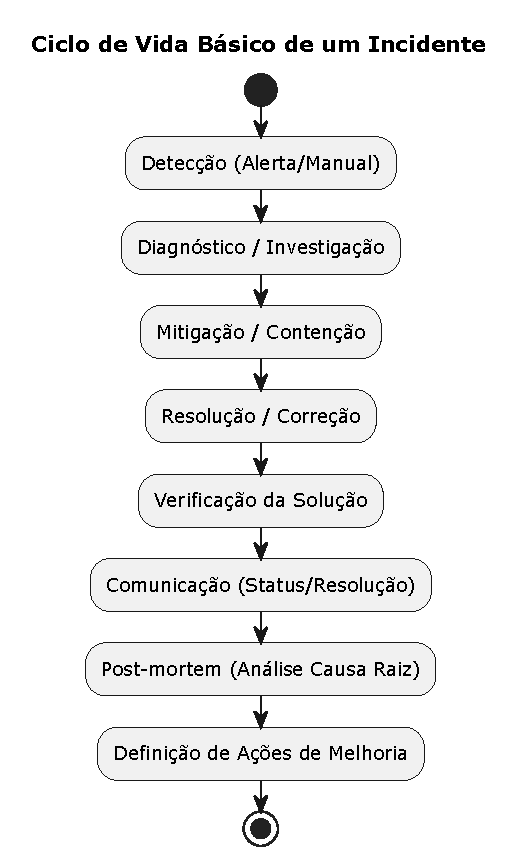
\includegraphics[width=0.9\textwidth]{assets/diagrama-ciclo-incidente.pdf}
    \caption{Ciclo de Vida Básico de um Incidente}
    \label{fig:ciclo-incidente}
\end{figure}

\begin{itemize}
    \item \textbf{Redução de MTTD (Mean Time To Detect):}
        \begin{itemize}
            \item \textbf{Alertas Acionáveis:} Garantir que os alertas configurados (baseados em SLOs e sintomas) sejam claros, relevantes e direcionem para a possível causa ou impacto. Evitar ruído excessivo de alertas não acionáveis.
            \item \textbf{Dashboards Consolidados (Grafana):} Manter dashboards que mostrem rapidamente a saúde dos serviços principais, o status dos SLOs e métricas chave, facilitando a identificação visual de anomalias.
            \item \textbf{Correlação:} Utilizar as ferramentas de observabilidade (Grafana com Loki/Jaeger/Prometheus) para correlacionar rapidamente métricas, logs e traces durante a investigação inicial.
        \end{itemize}
    \item \textbf{Redução de MTTR (Mean Time To Recover):}
        \begin{itemize}
            \item \textbf{Runbooks/Playbooks:} Documentar procedimentos passo-a-passo para diagnosticar e mitigar incidentes comuns ou alertas específicos. Devem ser mantidos atualizados e facilmente acessíveis.
            \item \textbf{Escalas de Plantão (On-Call):} Definir escalas de plantão claras, com responsabilidades bem definidas e ferramentas adequadas (PagerDuty/Opsgenie) para notificação e escalonamento.
            \item \textbf{Ferramentas de Comunicação:} Utilizar canais dedicados em ferramentas de chat (Slack, Teams) para comunicação focada durante um incidente ("War Room" virtual).
            \item \textbf{Automação de Mitigação (Opcional):} Para incidentes muito bem compreendidos, automatizar ações de mitigação (Exemplo: reiniciar um serviço específico, escalar temporariamente um recurso) via scripts ou ferramentas de automação.
            \item \textbf{Acesso e Permissões:} Garantir que a equipe on-call tenha o acesso necessário e seguro para investigar e aplicar correções nos ambientes.
            \item \textbf{Cultura de Post-mortems "Blameless":}
                \begin{itemize}
                    \item Realizar análises pós-incidente detalhadas para cada incidente significativo.
                    \item Foco em entender a \textbf{causa raiz sistêmica} (tecnologia, processo, monitoramento) e não em culpar indivíduos.
                    \item Documentar o incidente, a linha do tempo, o impacto, as ações tomadas e, principalmente, as \textbf{ações de acompanhamento} (melhorias no código, infraestrutura, monitoramento, runbooks) para prevenir recorrências.
                \end{itemize}
        \end{itemize}
\end{itemize}

\section{Feedback dos Clientes}
\label{sec:feedback-clientes}

A percepção do cliente é a medida final da confiabilidade. Coletar e agir sobre o feedback do cliente é essencial para complementar os dados técnicos de monitoramento.

\subsection{Canais de Coleta}
\label{subsec:canais-coleta}

\begin{table}[htbp]
    \centering
    \caption{Canais de Coleta de Feedback do Cliente}
    \label{tab:canais-coleta}
    \rowcolors{2}{gray!10}{white}
    % Usar tabularx e booktabs.
    \begin{tabularx}{\textwidth}{lX} % Removido '|'
        \toprule
        \textbf{Canal} & \textbf{Descrição / Exemplo} \\
        \midrule
        Pesquisas In-App/Web & Perguntas curtas sobre a experiência após ações chave (reserva, busca). \\
        Formulários de Contato/Suporte & Canal direto para reportar problemas ou dificuldades específicas. \\
        Análise de Chamados de Suporte & Categorizar e analisar os motivos dos contatos com a equipe de suporte. \\
        Monitoramento de Redes Sociais/Avaliação & Acompanhar menções à VOEBEM em plataformas públicas (Twitter, Reclame Aqui). \\
        Pesquisas de Satisfação (NPS/CSAT) & Medir a satisfação geral e a probabilidade de recomendação periodicamente. \\
        \bottomrule
    \end{tabularx}
\end{table}

\subsection{Processamento e Ação}
\label{subsec:processamento-feedback}

\textbf{Fluxo Básico de Tratamento de Feedback:}

\begin{figure}[htbp]
    \centering
    % Reduzindo a largura da imagem
    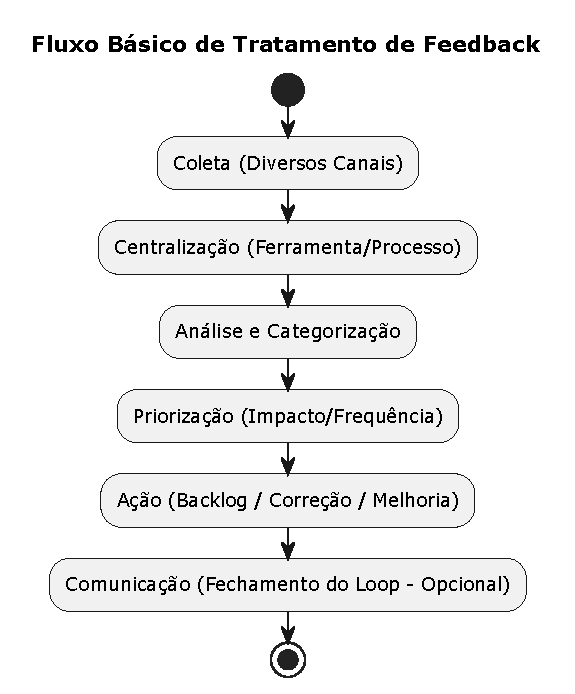
\includegraphics[width=0.9\textwidth]{assets/diagrama-fluxo-feedback.pdf}
    \caption{Fluxo Básico de Tratamento de Feedback}
    \label{fig:fluxo-feedback}
\end{figure}

\begin{itemize}
    \item \textbf{Centralização:} Agregar o feedback de diferentes canais em uma ferramenta ou processo unificado (Exemplo: um quadro Kanban, uma ferramenta de gestão de feedback).
    \item \textbf{Análise e Categorização:} Identificar temas recorrentes, problemas específicos, sugestões de melhoria. Correlacionar reclamações (Exemplo: lentidão) com dados de monitoramento técnico.
    \item \textbf{Priorização:} Avaliar o impacto e a frequência dos problemas reportados pelos clientes.
    \item \textbf{Integração com Backlog:} Transformar feedback acionável em itens de trabalho (bugs, melhorias) para as equipes de desenvolvimento e SRE.
    \item \textbf{Refinamento de SLIs/SLOs:} Usar o feedback para validar se os SLIs/SLOs atuais refletem a experiência real do usuário ou se novos indicadores são necessários (Exemplo: sucesso na conclusão do fluxo de reserva ponta-a-ponta).
    \item \textbf{Comunicação (Fechamento do Loop):} Informar aos clientes (quando apropriado e possível) sobre as ações tomadas com base em seus feedbacks, demonstrando que a empresa ouve e age.
\end{itemize}

% --- Final do Arquivo ---